\documentclass[conference]{IEEEtran}
\IEEEoverridecommandlockouts
\usepackage{fontspec}
\setmainfont{texgyretermes}[Extension=.otf,UprightFont=*-regular,BoldFont=*-bold,ItalicFont=*-italic,BoldItalicFont=*-bolditalic]
\usepackage{cite}
\usepackage{amsmath,amssymb,amsfonts}
\usepackage{graphicx}
\usepackage{booktabs}
\usepackage{xcolor}
\usepackage{tikz}
\usetikzlibrary{positioning,arrows.meta,fit,backgrounds,calc}
\usepackage[hidelinks]{hyperref}
\graphicspath{{figures/}}

\begin{document}

\title{SentriFormer: A Compact Multi-Task Encoder--Decoder Transformer Trained from Scratch for Complaint Routing, Satisfaction Estimation and Support-Reply Generation}

\author{
\IEEEauthorblockN{Author Name 1 (placeholder)}
\IEEEauthorblockA{\textit{Department (placeholder)} \\
\textit{Institution (placeholder)}\\
City, Country \\
email (placeholder)}
\and
\IEEEauthorblockN{Author Name 2 (placeholder)}
\IEEEauthorblockA{\textit{Department (placeholder)} \\
\textit{Institution (placeholder)}\\
City, Country \\
email (placeholder)}
\and
\IEEEauthorblockN{Author Name 3 (placeholder)}
\IEEEauthorblockA{\textit{Department (placeholder)} \\
\textit{Institution (placeholder)}\\
City, Country \\
email (placeholder)}
}

\maketitle

\begin{abstract}
Customer-support pipelines usually chain several large pre-trained models, one per task, which is costly to serve and hard to audit. We present SentriFormer, an 11.65M-parameter encoder--decoder Transformer trained from scratch on 3.54M customer-support records. Four lightweight heads on a shared, mean-pooled encoder perform 33-way complaint routing, 3-way sentiment, 5-level customer-satisfaction (CSAT) estimation and urgency scoring, while the decoder generates agent replies. We report the full development history under a pre-registered protocol: frozen acceptance criteria, matched control runs, bootstrap confidence intervals and a single use of the sealed test split per candidate. On 123,229 held-out complaints, the selected multi-task model routes with 73.7\% accuracy (majority baseline 27.2\%) and 0.737 weighted-F1. It reaches 88.1\% sentiment accuracy (0.758 macro-F1) and 72.4\% exact / 82.0\% within-one-star CSAT accuracy. Role-verified multi-turn training with a portal-redirect filter reduced replies that loop the customer back to a support portal from 31.3\% to 0.7\%. A further pre-registered reply filter cut broken-link replies from 5.8\% to 0.4\% and generic phrasing from 25.8\% to 16.6\% on fresh validation rows. We also document failure modes that matter in practice: shared-encoder drift under generation-only fine-tuning, routing collapse from class weights combined with label smoothing, and an urgency head that never beat a constant predictor. The model runs in 30\,ms per message for all classification heads and 275\,ms including reply generation on a laptop CPU.
\end{abstract}

\begin{IEEEkeywords}
multi-task learning, Transformer, customer support, complaint classification, response generation, data filtering, pre-registered evaluation
\end{IEEEkeywords}

\section{Introduction}
Organisations receive complaints through social media, web forms and regulators' portals. Each message must be routed to the right team, prioritised and answered. Current practice combines separate models: a fine-tuned encoder such as BERT~\cite{devlin2019bert} for classification, a sentiment model, and an increasingly large generator for replies~\cite{zhang2020dialogpt}. Each component brings its own pre-training corpus, licence, latency and failure modes, and the combination is difficult to evaluate end to end.

This paper asks a narrower question: \emph{how far can a single compact model, trained only on in-domain data, go on the core support tasks, and which training decisions actually move the numbers?} We answer it with SentriFormer, a 4+4-layer encoder--decoder Transformer~\cite{vaswani2017attention} with 11.65M parameters. It is pre-trained with T5-style span corruption~\cite{raffel2020exploring} on public complaint and customer-support corpora~\cite{twcs2017dataset,cfpbcomplaints} and then trained jointly on five outputs.

We do not claim a new architecture. SentriFormer uses standard Pre-LN blocks~\cite{xiong2020layer}, tied embeddings and hard parameter sharing~\cite{caruana1997multitask,ruder2017overview}. Our contributions are empirical and methodological:
\begin{enumerate}
\item A compact from-scratch multi-task model that handles routing, sentiment, CSAT and reply generation in one network, with sealed-test results for every development stage (Table~\ref{tab:test}).
\item A diagnosis of two silent failure modes and how each was repaired. In the first, generation-only fine-tuning moved the shared encoder and halved routing accuracy; a closed-form ridge map recovered it without gradients. In the second, the interaction of class weights with label smoothing collapsed the routing head.
\item A pre-registered study of dialogue-data interventions for support replies. Role verification, multi-turn context and targeted filters reduce portal-loop, broken-link and generic replies. Decoding-time (MMI) and weight-space interventions did \emph{not} pass, and we report these negative results in full.
\end{enumerate}

\section{Related Work}
\textbf{Encoder--decoder models and pre-training.} Sequence-to-sequence learning~\cite{sutskever2014sequence} and the Transformer~\cite{vaswani2017attention} underpin modern generation. BERT~\cite{devlin2019bert}, T5~\cite{raffel2020exploring} and BART~\cite{lewis2020bart} established pre-train-then-fine-tune at the 100M+ parameter scale. Compressed variants such as DistilBERT~\cite{sanh2019distilbert}, TinyBERT~\cite{jiao2020tinybert} and MobileBERT~\cite{sun2020mobilebert} reduce size but depend on a large teacher. Cramming~\cite{geiping2023cramming} and TinyStories~\cite{eldan2023tinystories} show that small models trained from scratch can be competitive when compute is limited or the domain is narrow. SentriFormer follows this from-scratch line in the customer-support domain.

\textbf{Multi-task learning.} Hard parameter sharing~\cite{caruana1997multitask,ruder2017overview} lets related tasks regularise each other, but can cause negative transfer~\cite{zhang2022survey}. Loss weighting by task uncertainty~\cite{kendall2018multitask} is one remedy; we use fixed weights and per-task sampling frequencies chosen on validation data.

\textbf{Class imbalance and calibration.} Label smoothing~\cite{szegedy2016rethinking} improves calibration but alters logit geometry~\cite{muller2019labelsmoothing}. Focal loss~\cite{lin2017focal} and class-balanced re-weighting~\cite{cui2019classbalanced} target long-tailed labels. We show that combining class weights with label smoothing in a common library implementation is harmful for a 33-class long-tailed routing task.

\textbf{Generic responses.} Maximum-likelihood dialogue models favour bland replies~\cite{vinyals2015neural,li2016diversity}. Proposed fixes include MMI decoding~\cite{li2016diversity}, nucleus sampling~\cite{holtzman2020curious}, unlikelihood training~\cite{welleck2020neural}, contrastive search~\cite{su2022contrastive} and data filtering by entropy~\cite{csaky2019improving} or connectivity~\cite{akama2020filtering}. Distinct-$n$ metrics mainly capture surface variation~\cite{tevet2021evaluating}, so we pair them with task-specific detectors.

\textbf{Customer support and complaints.} Xu et al.~\cite{xu2017new} and Hardalov et al.~\cite{hardalov2018towards} trained reply generators on Twitter support data. Complaint identification~\cite{preotiucpietro2019automatically,jin2020complaint} and CFPB product classification~\cite{oyewola2023consumer} are usually treated as separate tasks with separate models. We combine routing, satisfaction and generation in one model.

\textbf{Evaluation practice.} We use the bootstrap~\cite{efron1979bootstrap,koehn2004statistical} following significance-testing guidance for NLP~\cite{dror2018hitchhiker}, and pre-register acceptance criteria~\cite{vanmiltenburg2021preregistering}.

\section{Problem Formulation and Research Gap}
Given a customer message $x$, optionally with prior dialogue turns $h$, we want a single model $f_\theta$ that outputs: a routing label $y_r\in\{1..33\}$; a sentiment label $y_s\in\{\text{neg},\text{neu},\text{pos}\}$; a satisfaction estimate $y_c\in\{1..5\}$; an urgency score $y_u\in[0,3]$; and a reply $z$. All five outputs are produced in one forward pass and one decoding pass.

Three gaps motivate the work. (i) Prior support systems use one model per task and rarely report joint behaviour. (ii) Small from-scratch models are seldom evaluated on realistic, long-tailed support data. (iii) Reply-quality work mostly targets open-domain chat, where a reply that loops the customer back to a portal is not a failure; in support it is.

\section{Methodology}

\subsection{Architecture}
Fig.~\ref{fig:arch} and Table~\ref{tab:arch} summarise the model. Each encoder and decoder block applies LayerNorm before attention and before the feed-forward sub-layer~\cite{xiong2020layer}. Q/K/V/O projections have no bias and use scaled dot-product attention. The decoder applies an explicit causal mask together with a key-padding mask. One $16{,}000\times256$ embedding matrix is shared by the encoder, the decoder and the output projection. All classification heads read the masked mean of the final encoder states,
\begin{equation}
\bar{\mathbf{e}}=\frac{\sum_{t} m_t\,\mathbf{e}_t}{\sum_t m_t},
\end{equation}
followed by a $256\to256$ GELU projection and a task-specific linear layer. Sentiment and urgency share one projection trunk.

\begin{table}[t]
\centering
\caption{SentriFormer configuration (deployed checkpoint)}
\label{tab:arch}
\footnotesize
\setlength{\tabcolsep}{4pt}
\resizebox{\columnwidth}{!}{%
\begin{tabular}{@{}ll@{}}
\toprule
Property & Value \\
\midrule
Backbone & Encoder--decoder Transformer, 4 + 4 layers \\
$d_{\text{model}}$ / heads / head dim & 256 / 8 / 32 \\
Feed-forward & 1024, GELU, dropout 0.1 \\
Normalisation & Pre-LN (+ final LN), $\epsilon=10^{-6}$ \\
Positions & Fixed sinusoidal, 512 \\
Linear biases & None in backbone (heads keep bias) \\
Embedding & $16{,}000\times256$, tied enc/dec/LM head \\
Tokenizer & Byte-level BPE, 16k (106 special) \\
Heads (on mean-pooled encoder) & Routing 33, sentiment 3, CSAT 5, urgency 1 \\
Seq2seq core / total params & 11{,}447{,}296 / \textbf{11{,}654{,}698} \\
\bottomrule
\end{tabular}}
\end{table}


\begin{figure}[t]
\centering
\resizebox{\columnwidth}{!}{%
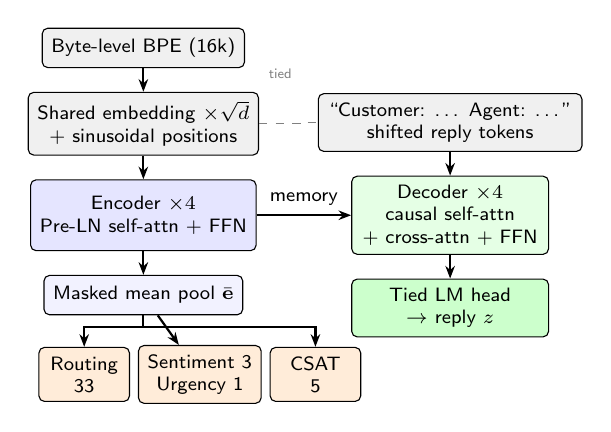
\begin{tikzpicture}[font=\sffamily\scriptsize, node distance=3mm,
 blk/.style={draw, rounded corners=2pt, minimum width=2.5cm, minimum height=5mm, align=center, fill=#1},
 blk/.default=white, ar/.style={-{Stealth[length=1.6mm]}, thick}]
\node[blk=gray!12] (tok) {Byte-level BPE (16k)};
\node[blk=gray!12, below=of tok] (emb) {Shared embedding $\times\sqrt{d}$\\+ sinusoidal positions};
\node[blk=blue!10, below=of emb, minimum height=9mm] (enc) {Encoder $\times4$\\ Pre-LN self-attn + FFN};
\node[blk=blue!5, below=of enc] (pool) {Masked mean pool $\bar{\mathbf e}$};
\node[blk=orange!15, below left=4mm and -11mm of pool, minimum width=1.15cm] (h1) {Routing\\33};
\node[blk=orange!15, right=1mm of h1, minimum width=1.15cm] (h2) {Sentiment 3\\Urgency 1};
\node[blk=orange!15, right=1mm of h2, minimum width=1.15cm] (h3) {CSAT\\5};
\node[blk=green!10, right=12mm of enc, minimum height=9mm] (dec) {Decoder $\times4$\\ causal self-attn\\ + cross-attn + FFN};
\node[blk=gray!12, above=of dec] (dctx) {``Customer: \dots\ Agent: \dots''\\ shifted reply tokens};
\node[blk=green!20, below=of dec] (lm) {Tied LM head\\ $\rightarrow$ reply $z$};
\draw[ar] (tok)--(emb); \draw[ar] (emb)--(enc); \draw[ar] (enc)--(pool);
\draw[ar] (pool.south)--++(0,-1.5mm)-|(h1.north); \draw[ar] (pool)--(h2); \draw[ar] (pool.south)--++(0,-1.5mm)-|(h3.north);
\draw[ar] (enc.east)--node[above]{memory}(dec.west); \draw[ar] (dctx)--(dec); \draw[ar] (dec)--(lm);
\draw[dashed, gray] (emb.east)-|($(dctx.west)+(-2mm,0)$)--(dctx.west);
\node[gray, font=\sffamily\tiny, above=0.5mm of emb.north east, anchor=south west] {tied};
\end{tikzpicture}}
\caption{SentriFormer. One encoder feeds four classification heads through a masked mean pool and conditions a decoder that generates the reply. The embedding is shared by encoder, decoder and LM head.}
\label{fig:arch}
\end{figure}

\subsection{Training objective}
Each optimiser step draws one mini-batch per task and minimises
\begin{equation}
\mathcal{L}=\mathcal{L}_{r}+0.3\,\mathcal{L}_{c}+0.3\,\mathcal{L}_{s}+0.5\,\mathcal{L}_{u}+\mathcal{L}_{d}.
\end{equation}
$\mathcal{L}_r$, $\mathcal{L}_c$ and $\mathcal{L}_s$ are cross-entropies with inverse-square-root class weights $w_k\propto n_k^{-1/2}$, normalised to mean 1, and no label smoothing. $\mathcal{L}_u$ is the squared error between $\sigma(\cdot)$ and $y_u/3$. $\mathcal{L}_d$ is the token-level cross-entropy of the reply, with EOS appended and padding ignored. CSAT and urgency batches are drawn every third and fourth step, respectively.

\subsection{Pre-registered development protocol}
Before any run, we froze written acceptance criteria: metric thresholds, the matched control run and bootstrap confidence intervals (CIs) computed with $B{=}1000$ resamples~\cite{efron1979bootstrap}. Candidates were selected on validation data. Each final candidate touched the sealed test split once. When a reply-quality candidate failed one criterion by a small margin, we pre-registered a replication on 500 new validation rows with unchanged thresholds before re-examining it. Fig.~\ref{fig:dev} shows the resulting development path.

\begin{figure*}[t]
\centering
\resizebox{\textwidth}{!}{%
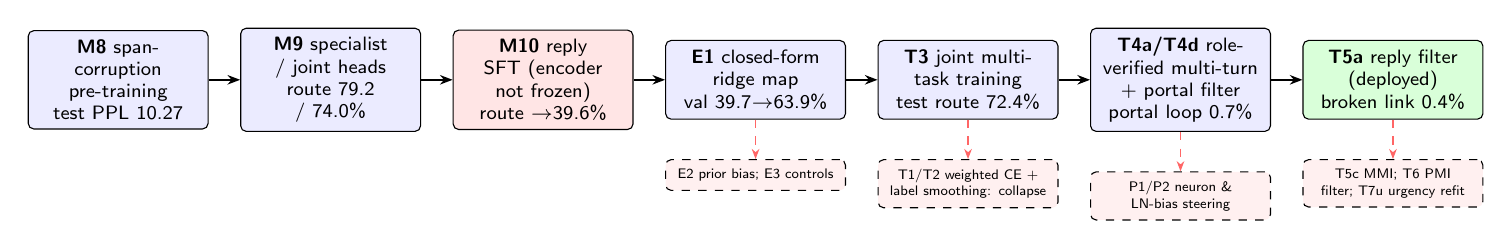
\begin{tikzpicture}[font=\sffamily\scriptsize, node distance=4mm,
 st/.style={draw, rounded corners=2pt, align=center, minimum height=10mm, text width=2.05cm, fill=#1},
 st/.default=blue!8, rj/.style={draw, dashed, rounded corners=2pt, align=center, text width=2.05cm, fill=red!6, font=\sffamily\tiny},
 ar/.style={-{Stealth[length=1.6mm]}, thick}, rr/.style={-{Stealth[length=1.3mm]}, red!60, dashed}]
\node[st] (m8) {\textbf{M8} span-corruption pre-training\\ test PPL 10.27};
\node[st, right=of m8] (m9) {\textbf{M9} specialist / joint heads\\ route 79.2 / 74.0\%};
\node[st=red!10, right=of m9] (m10) {\textbf{M10} reply SFT (encoder not frozen)\\ route $\rightarrow$39.6\%};
\node[st, right=of m10] (e1) {\textbf{E1} closed-form ridge map\\ val 39.7$\rightarrow$63.9\%};
\node[st, right=of e1] (t3) {\textbf{T3} joint multi-task training\\ test route 72.4\%};
\node[st, right=of t3] (t4) {\textbf{T4a/T4d} role-verified multi-turn + portal filter\\ portal loop 0.7\%};
\node[st=green!15, right=of t4] (t5) {\textbf{T5a} reply filter (deployed)\\ broken link 0.4\%};
\foreach \a/\b in {m8/m9,m9/m10,m10/e1,e1/t3,t3/t4,t4/t5} \draw[ar] (\a)--(\b);
\node[rj, below=5mm of e1] (e2) {E2 prior bias; E3 controls};
\node[rj, below=5mm of t3] (t12) {T1/T2 weighted CE + label smoothing: collapse};
\node[rj, below=5mm of t4] (p12) {P1/P2 neuron \& LN-bias steering};
\node[rj, below=5mm of t5] (t67) {T5c MMI; T6 PMI filter; T7u urgency refit};
\foreach \a/\b in {e1/e2,t3/t12,t4/p12,t5/t67} \draw[rr] (\a)--(\b);
\end{tikzpicture}}
\caption{Development history. Solid boxes were accepted under frozen criteria; dashed boxes were rejected. The red box marks the stage where routing collapsed, which E1 repaired.}
\label{fig:dev}
\end{figure*}

\subsection{Dialogue-data interventions}
\textbf{Role verification and multi-turn context (T4a).} We removed 52,424 training pairs whose ``agent'' target was actually written by a customer. Each remaining reply is conditioned on up to 256 tokens of role-labelled history (\texttt{Customer:}/\texttt{Agent:}).
\textbf{Portal filter (T4d).} We removed 65,198 pairs whose target only redirects the customer to a portal, a direct message or another channel.
\textbf{Reply filter (T5a).} We removed a further 29,483 replies flagged by rules: broken links left by URL stripping (24,610), whole-reply generic text, bulk personal-data requests and secret requests. We also removed 13 pairs identical across splits.

\section{Implementation and Experimental Setup}
\textbf{Data.} SentriCorpus merges the CFPB Consumer Complaint Database~\cite{cfpbcomplaints} (2.45M records), the Twitter customer-support corpus~\cite{twcs2017dataset} (1.05M), a Bitext support dataset (24k) and an e-commerce support dataset with CSAT survey scores (17k). Cleaning applies HTML unescaping, NFKC normalisation and whitespace collapsing. Exact duplicates are removed by SHA-256 hashing of normalised text. Records are assigned to splits deterministically by hashing their group (conversation, complaint cluster or order), giving a 90/5/5 split with no group shared across splits. Every supervised test row also lies in the pre-training test split. Table~\ref{tab:data} lists the task splits. Routing labels are the union of CFPB product and e-commerce category fields (33 classes; the largest class holds 27.2\% of the test rows). About 92\% of sentiment labels are teacher pseudo-labels; the rest come from a human-annotated emotion set, mapped to three classes.

\begin{table}[t]
\centering
\caption{Supervised splits derived from SentriCorpus (rows)}
\label{tab:data}
\footnotesize
\setlength{\tabcolsep}{3.2pt}
\resizebox{\columnwidth}{!}{%
\begin{tabular}{@{}lrrrl@{}}
\toprule
Task & Train & Val & Test & Label source \\
\midrule
Pre-training text & 3{,}184{,}956 & 176{,}586 & 177{,}169 & span corruption \\
Routing (33 cl.) & 2{,}219{,}168 & 122{,}961 & 123{,}229 & CFPB/e-com.\ product \\
CSAT (1--5) & 15{,}217 & 849 & 870 & post-contact survey \\
Sentiment (3 cl.) & 341{,}451 & 20{,}721 & 20{,}453 & teacher + human \\
Urgency (0--3) & 932 & 200 & 202 & public annot.\ set \\
Dialogue (multi-turn) & 479{,}445 & 28{,}454 & 28{,}907 & agent replies \\
\quad T4d filtered & 414{,}247 & -- & -- & portal filter \\
\quad T5a filtered & 384{,}751 & -- & -- & reply filter \\
\bottomrule
\end{tabular}}
\end{table}


\textbf{Tokenizer.} We trained a byte-level BPE tokenizer~\cite{sennrich2016neural} with NFKC normalisation and compared vocabularies of 16k, 24k and 32k. The 16k vocabulary averages 4.73 characters per token, produces no unknown tokens, and fits 96.73\% of texts within 512 tokens.

\textbf{Training and hardware.} Table~\ref{tab:hp} lists the optimisation settings. All runs used one NVIDIA RTX~3060 Laptop GPU (6\,GB) with 16\,GB RAM and seed 0. Phase-T runs peaked at 2.1--2.5\,GB of VRAM and took 0.19--0.23\,s per step.

\begin{table}[t]
\centering
\caption{Optimisation settings}
\label{tab:hp}
\footnotesize
\setlength{\tabcolsep}{3pt}
\resizebox{\columnwidth}{!}{%
\begin{tabular}{@{}lp{5.6cm}@{}}
\toprule
Stage & Setting \\
\midrule
Pre-training & AdamW, lr $5\!\times\!10^{-4}$, $\beta$=(0.9, 0.98), wd 0.01, cosine, 2k warm-up, batch 64, 149{,}200 steps (3 epochs), fp16, clip 1.0, 14.79 h \\
Phase T (T3) & AdamW; backbone lr $3\!\times\!10^{-5}$, heads $10^{-3}$; 2k-step frozen-backbone head warm-up; 18k steps; batches: routing 48, sentiment 32, dialogue 32, CSAT 16 (every 3rd step), urgency 8 (every 4th); 70.3 min, peak 2.23 GB VRAM \\
T4a--T6 & as T3, heads lr $3\!\times\!10^{-4}$, no head warm-up, dialogue context 256 tokens, 10k--18k steps \\
Selection & every 1k steps: $\text{acc}_{\text{route}}+\text{mF1}_{\text{csat}}+\text{mF1}_{\text{sent}}+\text{mF1}_{\text{urg}}-0.1\,\mathcal{L}_{\text{dial}}$ \\
Decoding & greedy, repetition penalty 1.2, $\le$100 new tokens \\
\bottomrule
\end{tabular}}
\end{table}


\textbf{Metrics.} We report accuracy, macro- and weighted-F1, and 15-bin expected calibration error (ECE) for classification. For CSAT we add within-one-star accuracy and MAE. For dialogue we report teacher-forced loss and perplexity, plus greedy generations on fixed contexts scored with ROUGE-L, distinct-$n$ and rule-based detectors (portal loop, broken link, generic phrase, action word). The detectors are regular expressions; their precision has not been audited by humans.

\section{Results and Discussion}

\subsection{Pre-training}
Span-corruption pre-training ran for 149,200 steps (14.79\,h). It reached a best validation loss of 2.425 and a test perplexity of 10.27, down from 16,445.75 at initialisation (Fig.~\ref{fig:pre}).

\begin{figure}[t]
\centering
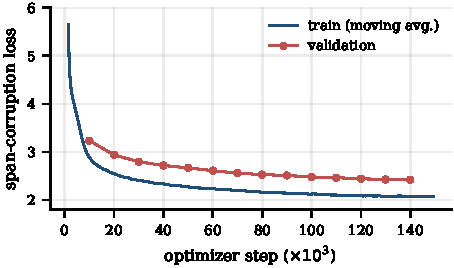
\includegraphics[width=\columnwidth]{pretrain_loss}
\caption{Span-corruption pre-training loss (moving average of training loss and periodic validation loss).}
\label{fig:pre}
\end{figure}

\subsection{Sealed-test results}
Table~\ref{tab:test} and Fig.~\ref{fig:hist} report the sealed test across stages. The single-task routing specialist (M9.2) remains the strongest router at 79.15\%. Multi-task models trade 5--6 points of routing accuracy for sentiment, CSAT and reply generation in the same 11.65M parameters. Among multi-task checkpoints, T4d is best or tied on routing (73.71\%, weighted-F1 0.737), sentiment (88.1\%, macro-F1 0.758) and dialogue perplexity (15.94). It also gives the lowest portal-loop rate (0.7\% against 31.3\% for T3; human agents in the reference replies loop 15\% of the time). Routing remains well calibrated (ECE 0.055; Fig.~\ref{fig:rel}). Only 0.5\% of messages fall below the 0.25-confidence threshold used to flag them for human triage. Truncating inputs to the 128 tokens used in deployment costs about 1.5 points.

\begin{table*}[t]
\centering
\caption{Sealed test-set results. Each checkpoint was scored on the test split exactly once, after selection on validation data. Routing at 512 tokens unless noted; $n$ = test rows. Best multi-task value in bold.}
\label{tab:test}
\footnotesize
\setlength{\tabcolsep}{4.2pt}
\resizebox{\textwidth}{!}{%
\begin{tabular}{@{}lcccccc|c@{}}
\toprule
Metric (test) & M9.2 specialist & M9.5 joint & M10.3 SFT & E1 ridge repair & T3 & T4d & Reference \\
\midrule
Routing accuracy (\%) ($n$=123{,}229) & 79.15 & 73.99 & 39.59 & 63.74 & 72.42 & \textbf{73.71} & majority 27.2 \\
Routing accuracy @128 tokens (\%) & 76.90 & 73.29 & 42.27 & 63.35 & 70.98 & \textbf{72.23} & -- \\
Routing macro-F1 / weighted-F1 & 0.404 / 0.789 & 0.317 / 0.734 & 0.078 / 0.388 & 0.205 / 0.618 & 0.353 / 0.725 & \textbf{0.369} / \textbf{0.737} & -- \\
Routing ECE (15 bins) & 0.051 & \textbf{0.048} & 0.165 & 0.069 & 0.058 & 0.055 & -- \\
CSAT exact / within-1 (\%) ($n$=870) & -- & 73.56 / 81.72 & 66.90 / 73.68 & \textbf{73.91} / \textbf{82.30} & 73.33 / 82.18 & 72.41 / 81.95 & -- \\
CSAT MAE / macro-F1 & -- & 0.732 / 0.317 & 1.030 / 0.278 & 0.717 / 0.311 & 0.714 / \textbf{0.361} & \textbf{0.708} / 0.352 & -- \\
Sentiment acc.\ (\%) / macro-F1 ($n$=20{,}453) & -- & -- & -- & -- & 87.2 / 0.742 & \textbf{88.1} / \textbf{0.758} & majority 79.6 \\
\quad human-labelled subset ($n$=3{,}012) & -- & -- & -- & -- & 61.6 / 0.531 & \textbf{63.7} / \textbf{0.552} & -- \\
Dialogue loss / perplexity ($n$=31{,}912) & -- & invalid$^\dagger$ & -- & -- & 2.782 / 16.14 & \textbf{2.769} / \textbf{15.94} & -- \\
Portal-loop replies, multi-turn (\%) & -- & -- & -- & -- & 31.3 & \textbf{0.7} & human agents 15 \\
ROUGE-L / distinct-2 (300 contexts) & -- & -- & -- & -- & \textbf{0.135} / 0.209 & 0.132 / \textbf{0.235} & -- \\
\bottomrule
\multicolumn{8}{@{}l}{\scriptsize $^\dagger$M9.5 reported a perplexity of 1.04 caused by a causal-mask leak; it is excluded. The specialist M9.2 has no other heads trained. Urgency is reported separately in Section~\ref{sec:neg}.}
\end{tabular}}
\end{table*}


\begin{figure}[t]
\centering
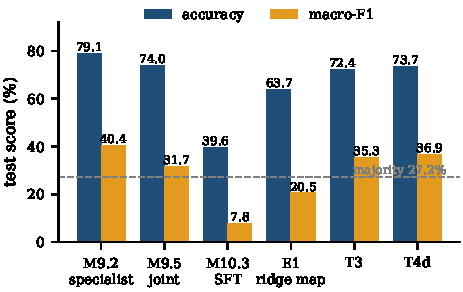
\includegraphics[width=\columnwidth]{history_category}
\caption{Sealed-test routing accuracy and macro-F1 across development stages (123,229 complaints). The dashed line is the majority-class rate.}
\label{fig:hist}
\end{figure}

\textbf{Per-class behaviour.} Fig.~\ref{fig:pc} shows that well-populated products reach high F1 (mortgage 0.91, student loan 0.84, checking/savings 0.80, debt collection 0.78). Twelve of the 33 classes score F1 = 0. Most of these are e-commerce categories with 1--40 test rows, or CFPB legacy labels that duplicate a newer label (three credit-reporting and three payday-loan variants). The resulting confusion between duplicate labels lowers macro-F1 but is largely harmless for routing.

\begin{figure}[t]
\centering
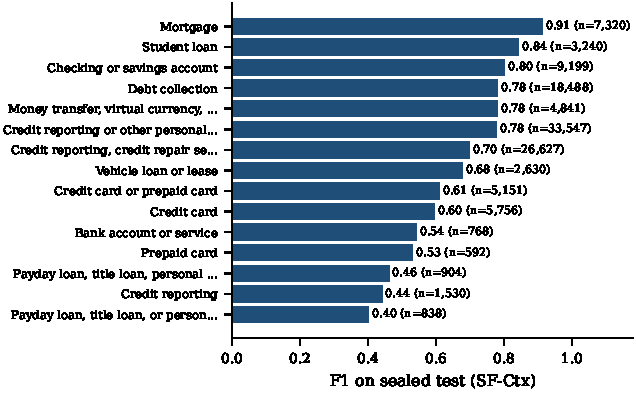
\includegraphics[width=\columnwidth]{perclass_f1}
\caption{Per-class sealed-test F1 of T4d for classes with at least 500 test rows.}
\label{fig:pc}
\end{figure}

\textbf{Sentiment and CSAT.} Sentiment is strong on teacher-labelled rows (92.3\% accuracy) but weaker on the human-labelled subset (63.7\%, macro-F1 0.552), which reflects a distribution shift from support text to general emotional text. CSAT predictions concentrate on 1 and 5 stars (Fig.~\ref{fig:cm}). The model almost never predicts 2 stars, so the 2- and 3-star classes have near-zero F1. Within-one-star accuracy (82\%) is the more useful operating metric.

\begin{figure}[t]
\centering
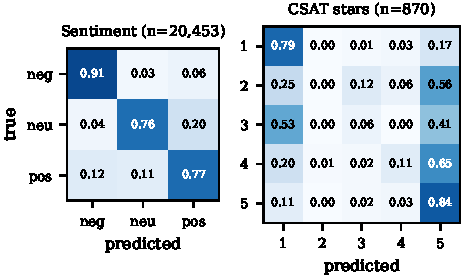
\includegraphics[width=\columnwidth]{confusion_sent_csat}
\caption{Row-normalised sealed-test confusion matrices of T4d for sentiment and CSAT.}
\label{fig:cm}
\end{figure}

\begin{figure}[t]
\centering
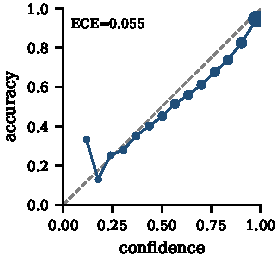
\includegraphics[width=0.55\columnwidth]{reliability}
\caption{Routing reliability diagram (T4d test). Marker size is proportional to bin count.}
\label{fig:rel}
\end{figure}

\subsection{Failure modes and their repair}
\textbf{Shared-encoder drift.} The M10 reply fine-tuning froze the task heads but not the shared encoder and embeddings. The relative embedding drift reached 66\%, and sealed-test routing fell from 73.99\% to 39.59\% (paired-bootstrap difference $-34.4$\,pp, 95\% CI $[-34.7,-34.1]$). Phase~0 (E1) repaired it without gradients. We fitted a ridge map $A\in\mathbb{R}^{256\times256}$ from the drifted pooled features to the pre-drift features on 200k training rows ($R^2=0.674$) and folded it into the first layer of the routing and CSAT heads. Validation routing recovered from 39.67\% to 63.94\%. Two controls, a random edit of equal norm (21.9\%) and a map fitted to shuffled pairs (27.4\%), fell far short, so the gain comes from the fitted map rather than from editing the head weights at all.

\textbf{Weighted label smoothing.} T1 combined class weights with label smoothing 0.1. In the library implementation, the class weights also scale the smoothing term, which pushes every prediction toward heavily weighted rare classes. Validation routing dropped from 64\% to 36\%. An offline probe isolated the cause: plain cross-entropy gave 65.3\%, weights with smoothing 36\%, and weights without smoothing 63.8\%. T3 removed the smoothing and recovered to 72.7\% validation and 72.4\% test accuracy. Fig.~\ref{fig:curves} shows that Phase-T training was stable once this was fixed.

\begin{figure}[t]
\centering
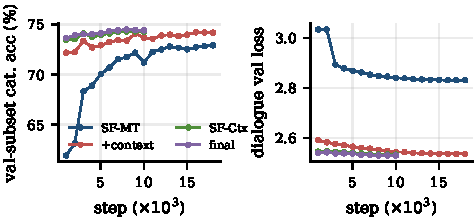
\includegraphics[width=\columnwidth]{phaseT_curves}
\caption{Phase-T validation-subset routing accuracy and dialogue loss during training.}
\label{fig:curves}
\end{figure}

\subsection{Reply quality of the deployed model}
T5a, the deployed checkpoint, starts from T4d and trains on the T5a-filtered data. Its control run, T5a-ctrl, trains for the same number of steps on unfiltered data. In the first test on 500 validation rows, T5a cut broken-link replies from 3.0\% to 0.8\% (CI against the control $[-3.8,-0.8]$\,pp) and generic phrasing from 26.8\% to 17.2\%. It still failed one pre-registered gate: the action-word rate fell by 2.2\,pp against a limit of 2.0\,pp, and that CI included zero. In the pre-registered replication on 500 new rows (Fig.~\ref{fig:rq}), every gate passed. Broken-link replies fell from 5.8\% to 0.4\% (CI against the control $[-6.2,-2.6]$\,pp), generic phrasing from 25.8\% to 16.6\% (CI $[-12.6,-5.8]$\,pp), and whole-reply generic text from 14.8\% to 7.4\%, while the action-word rate held (39.6\%$\rightarrow$40.2\%). Classification heads moved by at most 0.9\,pp on validation (Table~\ref{tab:val}). T5a has not yet been scored on the sealed test; the test numbers in Table~\ref{tab:test} are those of its parent, T4d.

\begin{figure}[t]
\centering
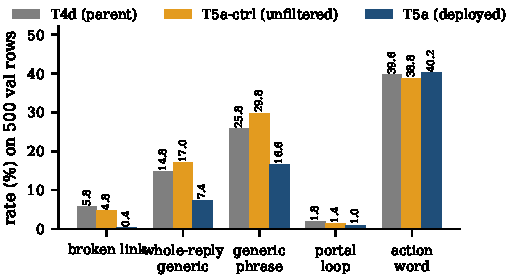
\includegraphics[width=\columnwidth]{reply_quality_t5a}
\caption{Rule-detected reply properties in the pre-registered replication (500 fresh validation rows, greedy decoding). Lower is better except for action words.}
\label{fig:rq}
\end{figure}

\begin{table}[!t]
\centering
\caption{Validation metrics of the training stages ($n$: routing 122{,}961, CSAT 849, sentiment 20{,}721)}
\label{tab:val}
\footnotesize
\setlength{\tabcolsep}{2.6pt}
\resizebox{\columnwidth}{!}{%
\begin{tabular}{@{}lccccc@{}}
\toprule
Run & Route acc & Route mF1 & CSAT mF1 & Sent mF1 & Dial.\ loss \\
\midrule
Closed-form repair & 63.94 & 0.209 & 0.302 & 0.265$^\ast$ & 2.984 \\
SF-MT & 72.71 & 0.371 & 0.318 & 0.743 & 2.782 \\
+ role-verified context & 73.84 & 0.385 & 0.328 & 0.758 & 2.765 \\
SF-Ctx (+ portal filter) & 74.03 & 0.386 & \textbf{0.336} & 0.763 & 2.770 \\
Control (same steps, no filter) & \textbf{74.22} & \textbf{0.387} & 0.333 & \textbf{0.764} & \textbf{2.764} \\
\textbf{SentriFormer (final)} & 73.37 & 0.377 & 0.330 & 0.756 & 2.780 \\
PMI filter (rejected) & 74.02 & 0.385 & 0.327 & 0.761 & 2.778 \\
\bottomrule
\multicolumn{6}{@{}l}{\scriptsize $^\ast$untrained sentiment head.}
\end{tabular}}
\end{table}


\subsection{Negative results}\label{sec:neg}
Table~\ref{tab:neg} lists the rejected interventions. None of the weight-space edits (P1, P2) or the decoding change (T5c) beat matched random controls. Because generic replies were not concentrated in a few neurons, filtering the training data was the intervention that worked. The PMI filter (T6) removed 64k more replies without improving relevance. The urgency head is the clearest negative result. It beats the majority class in macro-F1 (0.376 vs.\ 0.148), but its MAE is worse than predicting the mean (0.691 vs.\ 0.675 on test). A logistic probe on the frozen encoder reaches only 0.35 macro-F1, so the problem is likely the 932 training labels, whose provenance is unknown. Urgency should be treated as untrained.

\begin{table}[!t]
\centering
\caption{Interventions rejected under pre-specified criteria (validation only)}
\label{tab:neg}
\footnotesize
\setlength{\tabcolsep}{2.5pt}
\resizebox{\columnwidth}{!}{%
\begin{tabular}{@{}p{3.3cm}p{4.6cm}@{}}
\toprule
Intervention & Outcome against matched controls \\
\midrule
Class-weighted CE + label smoothing 0.1 & routing collapsed 64\%$\rightarrow$36\%; stop gate failed \\
Gradient-free class-prior bias edit & +1.6 pp accuracy, but 8 key classes lost $>$2 pp \\
Scaling 4 ``generic'' decoder FFN neurons & no effect beyond 5 random-neuron controls \\
Adding a ``generic'' direction to a LayerNorm bias & matched by random directions; action words 38.4$\rightarrow$30.4\% \\
MMI re-ranking of 8 sampled replies & a random pick beat MMI; more broken links \\
PMI$<$0 reply filter (64k more rows removed) & relevance gain CI includes 0; action words $-$4.4 pp \\
Re-fitting the urgency projection & MAE 0.752 vs.\ 0.671 for a mean predictor \\
\bottomrule
\end{tabular}}
\end{table}


\subsection{Inference cost}
On 30 benchmark complaint messages (4--58 words, two repetitions each), all classification heads plus one decoding step take a median of 30.4\,ms on a laptop CPU (8 PyTorch threads) and 59.4\,ms on the RTX~3060. A full analysis with a greedy reply of up to 100 tokens (16.3 words on average) takes 275\,ms on the CPU (p95 502\,ms) and 586\,ms on the GPU. At batch size one the model is small enough that GPU kernel-launch overhead outweighs the compute, which is why the CPU is faster. The checkpoint is 46.7\,MB.

\section{Limitations and Future Scope}
(i) No human evaluation of replies has been completed. Reply metrics rely on regex detectors without a precision audit and on ROUGE-L ($\approx$0.13). (ii) The deployed T5a lacks its own sealed-test run. (iii) All Phase-T results come from a single seed, and test differences between T3 and T4d have no CIs. (iv) We did not train classical (TF-IDF + logistic regression) or pre-trained (DistilBERT, T5-small) baselines on the same splits, so we cannot claim superiority over them. (v) Sentiment labels are mostly pseudo-labels; CSAT is trained on e-commerce remarks but applied to financial complaints; urgency and escalation are not learned. (vi) De-duplication is exact-hash only, and the Twitter corpus licence is non-commercial. Future work: a blinded human A/B study, merging duplicate CFPB labels into a hierarchical taxonomy, human-labelled urgency data, multi-seed runs with matched baselines, and retrieval grounding of replies in policy text.

\section{Conclusion}
SentriFormer shows that one 11.65M-parameter model trained from scratch on in-domain data can route complaints at 73.7\% accuracy over 33 classes, estimate sentiment and satisfaction, and draft support replies, all within about 0.3\,s on a laptop CPU. The largest gains came from training-data decisions: removing label smoothing, adding role-verified context, and filtering portal-redirect and broken-link replies. Architectural or decoding tricks contributed little. A pre-registered protocol with matched controls was essential to tell real gains from noise. It also exposed failures, such as encoder drift and an untrainable urgency head, that would otherwise have gone unreported.

\section*{Acknowledgment}
[Acknowledgment placeholder: supervisors, institution and funding, to be supplied by the authors.]

\bibliographystyle{IEEEtran}
\bibliography{references}

\end{document}
